\section{Tecnologie utilizzate}
\label{tec_utilizzate}
In questa sezione verranno presentate le tecnologie su cui si basa lo sviluppo del progetto. In particolare, si presterà attenzione alle motivazioni per cui si è deciso di adottarle.

	\subsection{C++}
	\label{c++}
	Si è deciso di sviluppare \project{} con il linguaggio di programmazione C++. Questa scelta è stata dettata prevalentemente dai seguenti motivi:
	\begin{itemize}
		\item\textbf{Librerie consigliate:} le librerie a cui appoggiarsi per semplificare alcune attività, indicate dai proponenti, sono scritte in questo linguaggio. Il campo di applicazione di tali librerie verrà esposto in seguito;
		\item\textbf{Conoscenza del linguaggio:} la totalità dei componenti del gruppo, ha già avuto una buona dose di esperienza con tale linguaggio. Questo aspetto, sommato al precedente, è stato considerato sufficiente per giustificare questa scelta.
	\end{itemize}
	
	\subsection{Qt}
	\label{qt}
	Si è deciso di utilizzare il framework\glossario{} Qt\glossario{} per lo sviluppo delle classi dell'architettura. Questa scelta è stata fatta perché Qt\glossario{} offre i seguenti vantaggi:
	\begin{itemize}
	\item\textbf{Framework C++:} Qt\glossario{} è un framework\g{} basato principalmente sul linguaggio C++\glossario{};
	\item\textbf{Forte componente grafica:} tale framework\glossario{} è notoriamente orientato ad una particolare cura verso l'aspetto front-end delle applicazioni. Data l'importanza della GUI\glossario{} nel progetto \project, Qt\glossario{} è stato considerato adeguato per lo sviluppo.
	\item\textbf{Qt Designer:} applicativo che permette di disegnare interfacce grafiche senza agire direttamente sul codice sorgente. È possibile creare e personalizzare le finestre in modalità \lq\lq{}what-you-see-is-what-you-get\rq\rq{}. Inoltre, tutti gli oggetti creati (Widgets, forms, ecc\dots) si integrano con il codice sorgente usando il meccanismo di \textit{Signals \& Slots}\glossario{}, per cui diventa facile assegnare i comportamenti agli elementi grafici;
	\item\textbf{Qt Creator:} IDE\glossario{} multipiattaforma per lo sviluppo di applicazioni Qt\glossario{}. Esso integra il controllo di versione appoggiandosi anche a Git\glossario{};
	\item\textbf{Esperienza del gruppo:} tutti i componenti hanno già avuto contatto con il framework\glossario{}. Questa scelta mira anche a minimizzare il tempo di studio individuale delle tecnologie.
	\end{itemize}
	
	\subsubsection{Signals \& Slots}
	\label{signalslot}
	Il meccanismo di \textit{Signals \& Slots}\glossario{}, è una caratteristica fondamentale del framework\g{} Qt\glossario{} che si occupa di far comunicare tra di loro gli oggetti.\\
	Questo aspetto è determinante nel momento in cui si vuole sviluppare una GUI\glossario{}, dato che ad un'azione che l'utente compie sull'interfaccia grafica, molto probabilmente ne consegue un'operazione nella parte logica dell'applicativo e viceversa. Più generalmente, si vogliono far comunicare due o più oggetti di qualsivoglia tipo. Tutte le classi derivate da \textbf{QObject} (classe base del framework\glossario{}), possono contenere \textit{Signals}\glossario{} e \textit{Slots}\glossario{}.
	\\In Qt\glossario{}, viene emesso un \textit{Signal}\glossario{} nel momento in cui avviene un particolare evento. Le classi derivate da \textbf{QWidget} (è la classe base da cui derivano tutti gli oggetti grafici) hanno \textit{Signals}\glossario{} predefiniti, ma è sempre possibile creare delle sottoclassi che ereditano dalle precedenti ed implementare i \textit{Signals}\glossario{} che si desiderano. Gli \textit{Slots}\glossario{} sono delle funzioni che vengono invocate in risposta ad un particolare \textit{Signal}\glossario{}. Anche in questo caso, alcune classi hanno degli \textit{Slots}\glossario{} predefiniti, ma è possibile crearne di personalizzati ereditando le classi opportune.
	Per collegare il \textit{Signal}\glossario{} di un oggetto con lo \textit{Slot}\glossario{} di un altro, è necessario utilizzare la primitiva (vedi fig. \ref{signalimg}):
	\begin{verbatim}
					connect(Object_x, signal_1, Object_y, slot_2)
	\end{verbatim}
	\begin{figure}[!h]
		\centering
		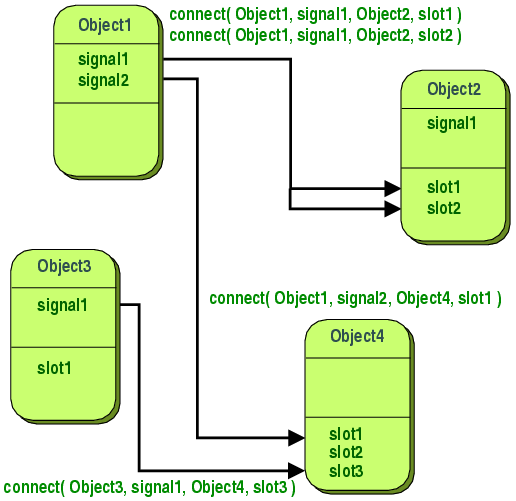
\includegraphics[scale=0.5]{./Content/Immagini/SignalSlot}
		\caption{Schema interazione oggetti tramite \textit{Signals \& Slots}}
		\label{signalimg}
	\end{figure}
	Questo meccanismo è \textit{type safe}: la segnatura del \textit{Signal}\glossario{} deve combaciare con la segnatura dello \textit{Slot}\glossario{} ad esso associato. Inoltre queste due entità sono estremamente disaccoppiate, nel senso che l'oggetto emettente il \textit{Signal}\glossario{}, non si preoccupa del fatto che verrà raccolto o meno e di chi lo raccoglierà. La responsabilità è completamente spostata sullo sviluppatore.
	
	\subsubsection{The Meta-Object System}
	\label{mos}
	Il \textit{Meta-Object System} fornisce il meccanismo di \textit{Signals \& Slots}\glossario{} di Qt\glossario{} ed inoltre, offre supporto per l'RTTI\glossario{} (RunTime Type Identification) e per altre operazioni eseguite dinamicamente. Il sistema si basa su tre componenti fondamentali:
	\begin{enumerate}
	\item\textbf{QObject:} è una classe che funge da classe-base per oggetti che possono sfruttare il sistema;
	\item\textbf{Q\_OBJECT:} è una macro inserita all'interno della sezione privata della dichiarazione di una classe. È usata per abilitare le funzioni dei Meta-Oggetti, quali RTTI (RunTime Type Information)\glossario{}, \textit{Signals}\glossario{} e \textit{Slots}\glossario;
	\item\textbf{MOC (\textbf{The Meta-Object Compiler}):} è un pre-processore che fornisce ad ogni sottoclasse di \verb!QOject!, il codice sorgente necessario ad implementare le caratteristiche dei Meta-Oggetti.
	\end{enumerate}
	Il MOC legge i sorgenti C++. Se trova uno o più dichiarazioni di classe che contengono la macro \verb!Q_OBJECT!, produce un sorgente C++ contenente il codice dei Meta-Oggetti, per ognuna di queste classi. Questi file generati dal MOC, possono essere inclusi nei sorgenti da cui derivano (tramite le direttive di \verb!#include! inserite automaticamente) oppure, più usualmente, vengono compilati e linkati con le implementazioni delle classi.
	
	\subsubsection{Licenza}
	\label{licenza}
		Il framework\g{} Qt\glossario{} viene distribuito sotto tre diverse tipologie di licenze, in maniera da andare incontro alle esigenze dei vari team di sviluppo.
		\begin{itemize}
		\item Una versione commerciale, di proprietà del \textbf{Qt Digia}, adatta per sviluppare software proprietario anche a fini commerciali, in cui non è previsto il rilascio del codice sorgente;
		\item La licenza \textbf{LGPL v2.1 (\textit{GNU Lesser General Public License})}\footnote{\url{https://qt-project.org/doc/qt-5.0/qtdoc/lgpl.html}}. \`E una licenza di software libero, che permette alle classi della libreria di essere linkate da codice non libero;
		\item La licenza \textbf{GPL v3.0 (\textit{GNU General Public License})}\footnote{\url{https://qt-project.org/doc/qt-5.0/qtdoc/gpl.html}}. \`E una licenza di software libero che garantisce all'utente la libertà di utilizzo, copia, modifica e distribuzione del prodotto. Permette inoltre di integrare il progetto con le librerie dotate di licenza ad essa compatibile. Dato che le altre librerie con cui si svilupperà \project{}, sono licenziati compatibilmente con la GPL, si è deciso di adottare Qt\glossario{} con questa licenza.
	\end{itemize}
	
	\subsection{ITK}
	\label{itk}
		Si è deciso di utilizzare la libreria ITK\glossario{}, per implementare alcune operazioni fondamentali che il software deve svolgere. In particolare, fornisce delle classi che permettono di importare svariate tipologie di formati di immagini nel sistema e conseguentemente di esportarle. Inoltre, sono disponibili delle classi che consentono di memorizzare degli algoritmi che operano sulle immagini (chiamate filtri). Quest'ultima caratteristica risulta fondamentale per implementare le feature extractors\glossario{} e gli algoritmi di clustering\glossario{}.\\
		ITK\glossario{} è stato scelto principalmente per i seguenti motivi:
		\begin{itemize}
		\item Indicazione dei proponenti;
		\item Libreria interamente scritta in C++ e quindi facilmente integrabile con Qt\glossario{};
		\item Libreria ideata per operare su dati biomedici; integra quindi la possibilità di manipolare immagini e dati provenienti da fMRI\glossario{} ecc\dots{};
		\item Fornita con licenza Apache v2.0, una licenza di software libero compatibile con la GPL v3.0;
		\item Libreria multipiattaforma.
	\end{itemize}
	
	\subsection{VTK}
	\label{vtk}
		Si è deciso di utilizzare la libreria VTK\glossario{}, per implementare le funzioni di visualizzazione delle immagini biomediche che il software dovrà supportare. In particolare, fornisce delle classi che permettono di manipolare immagini con formato Analyze 7.5\glossario{} e NIfTI\glossario{} e di poterle quindi importare e visualizzare.\\
		VTK\glossario{} è stato scelto principalmente per i seguenti motivi:
		\begin{itemize}
		\item Indicazione dei proponenti;
		\item Libreria interamente scritta in C++ e compatibile con Qt\glossario{};
		\item Libreria multipiattaforma;
		\item Ideata per operare su dati biomedici.
		\end{itemize}
		
	\subsection{OpenCV}
	\label{opencv}
	Si è deciso di utlizzare la libreria OpenCV\footnote{http://opencv.org} per leggere i video in formato 2D e per convertirli in immagini in formato ITK\g{}.
	\\OpenCV è stata scelta principalmente per i seguenti motivi:
		\begin{itemize}
			\item Libreria scritta in linguaggio C++ e quindi facilmente integrabile;
			\item Si tratta di una libreria multipiattaforma.
		\end{itemize}
	
	\subsection{SQLite}
	\label{sqlite}
	Per implementare il database su cui il software andrà ad operare, si è deciso di utilizzare SQLite. Quest'ultima è una libreria software scritta in linguaggio C, che definisce un DBMS SQL incorporabile all'interno di applicazioni.\\
	Le principali motivazioni che hanno portato a questa scelta sono:
	\begin{itemize}
	\item SQLite supporta la specifica standard SQL 92, di cui ogni componente del gruppo ha già avuto esperienza;
	\item L'installazione è compatta e leggera, infatti occupa solo 256KB di memoria;
	\item È autosufficiente, nel senso che non necessita di un server;
	\item È una libreria di dominio pubblico;
	\item Offre il vantaggio di memorizzare l'intero database in un unico file. In questo modo SQLite non diffonde files all'interno del calcolatore portando a dei benefici in termini di memoria occupata.
	\end{itemize}